\section*{Problem 2}
	\begin{enumerate} [1)]
		\item \begin{proof} [Solution]
			Here is the result. I use uniform samples for $X_i$. The below graph shows log-scale axis with number of samples versus errors. This graph has slope -1. i.e. The value $\alpha = -1$, rate of convergence is $O\left(\frac{1}{N}\right)$.
			\begin{center}
				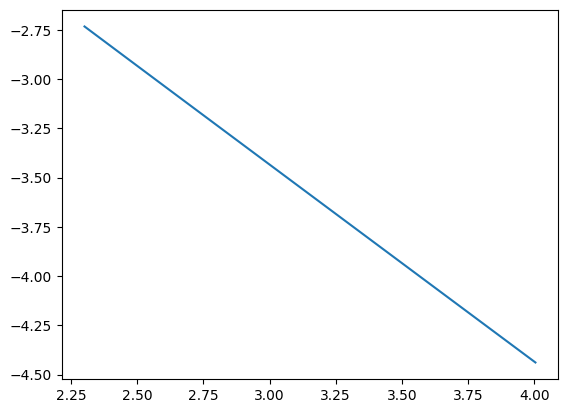
\includegraphics[width=0.4\textwidth]{line_with_-1.png}
			\end{center}
		\end{proof}
		\item \begin{proof} [Solution]
			Here is the result. The blue dots represent $\mu_M(N)$ for each $M$ and the orange line has slope $-\frac{1}{2}$. Note that this also has the similar log-scale axis. It shows that $\mu_M$ also converges, but not as fast as the above problem. Because it has the rate of convergence $O\left(\frac{1}{\sqrt{N}}\right)$.
			\begin{center}
				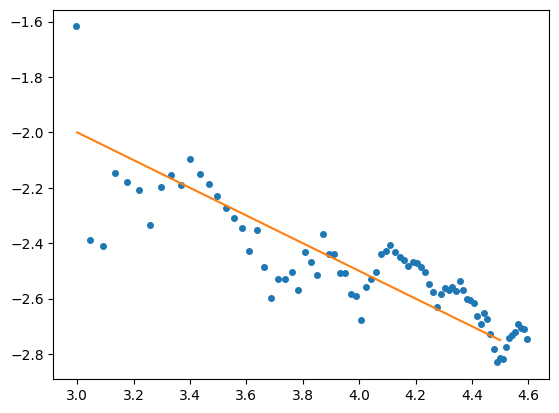
\includegraphics[width=0.4\textwidth]{line_with_half.png}
			\end{center}
		\end{proof}
	\end{enumerate}